\documentclass[tikz,border=8pt]{standalone}
\usepackage{xcolor}
\usetikzlibrary{calc,arrows.meta,backgrounds}
\definecolor{bg}{HTML}{1B1F27}
\definecolor{fg}{HTML}{E6EDF3}
\definecolor{dim}{HTML}{9AA5B1}
\definecolor{cx}{HTML}{E5826F}
\definecolor{cy}{HTML}{7BC47F}
\definecolor{cz}{HTML}{6EA8FE}
\definecolor{feat}{HTML}{F0C060}
\definecolor{c1}{HTML}{7BC47F}
\definecolor{c2}{HTML}{E5826F}
\begin{document}
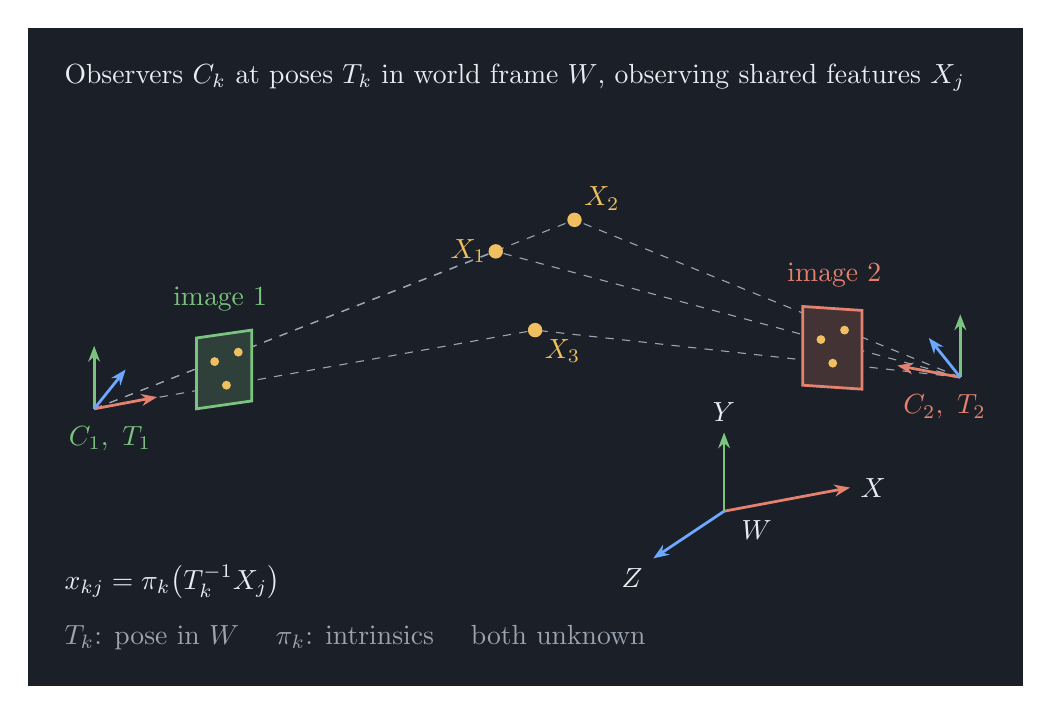
\begin{tikzpicture}[show background rectangle, background rectangle/.style={fill=bg}, inner frame sep=10pt, every node/.style={text=fg}, ax/.style={-{Stealth[length=2mm]}, line width=1pt}]
\coordinate (W) at (8.5,0.9);
\coordinate (C1) at (0.5,2.2);
\coordinate (C2) at (11.5,2.6);
\coordinate (X1) at (5.6,4.2);
\coordinate (X2) at (6.6,4.6);
\coordinate (X3) at (6.1,3.2);

\foreach \f in {X1,X2,X3}{
  \draw[dim, dashed] (C1) -- (\f);
  \draw[dim, dashed] (C2) -- (\f);
}

\draw[ax, cx] (W) -- ++(1.6,0.3) node[right] {$X$};
\draw[ax, cy] (W) -- ++(0,1.0) node[above] {$Y$};
\draw[ax, cz] (W) -- ++(-0.9,-0.6) node[below left] {$Z$};
\node[anchor=north west] at ($(W)+(0.1,0)$) {$W$};

\draw[fill=c1!20!bg, draw=c1, line width=1pt] (1.8,2.2) -- (2.5,2.3) -- (2.5,3.2) -- (1.8,3.1) -- cycle;
\node[text=c1] at (2.1,3.6) {image 1};
\draw[fill=c2!20!bg, draw=c2, line width=1pt] (9.5,2.5) -- (10.25,2.45) -- (10.25,3.45) -- (9.5,3.5) -- cycle;
\node[text=c2] at (9.9,3.9) {image 2};

\foreach \f in {X1,X2,X3}{
  \fill[feat] ($(C1)!0.3!(\f)$) circle (1.6pt);
  \fill[feat] ($(C2)!0.3!(\f)$) circle (1.6pt);
  \fill[feat] (\f) circle (2.6pt);
}
\node[text=feat, left] at (X1) {$X_1$};
\node[text=feat, above right] at (X2) {$X_2$};
\node[text=feat, below right] at (X3) {$X_3$};

\draw[ax, cx] (C1) -- ++(0.8,0.15);
\draw[ax, cy] (C1) -- ++(0,0.8);
\draw[ax, cz] (C1) -- ++(0.4,0.5);
\node[text=c1, below] at ($(C1)+(0.2,-0.1)$) {$C_1,\ T_1$};
\draw[ax, cx] (C2) -- ++(-0.8,0.15);
\draw[ax, cy] (C2) -- ++(0,0.8);
\draw[ax, cz] (C2) -- ++(-0.4,0.5);
\node[text=c2, below] at ($(C2)+(-0.2,-0.1)$) {$C_2,\ T_2$};

\node[anchor=west] at (0,6.4) {Observers $C_k$ at poses $T_k$ in world frame $W$, observing shared features $X_j$};
\node[anchor=west] at (0,0) {$x_{kj}=\pi_k\!\left(T_k^{-1}X_j\right)$};
\node[anchor=west, text=dim] at (0,-0.7) {$T_k$: pose in $W$ \quad $\pi_k$: intrinsics \quad both unknown};
\end{tikzpicture}
\end{document}
